% !TeX root = ../dlvc.tex
\newcommand{\ttitle}{Image Classification with CNN}
\hyphenation{}
\maketitle
%\keywords{stochastic gradient descent, convolutional neural network, softmax, multilayer perceptron}
\begin{abstract}
This is the report for the third assignment of the course ``Deep Learning for Visual Computing'' in the winter term 2016 at the TU Vienna. The task was to improve the missclassification rate of images of  the CIFAR10~\cite{CIFAR10} dataset by training data augmentation and a better architecture for the neural net.
\end{abstract}

\section{Deep Learning Libraries}
% Briefly state which deep learning library you used and if you used the server for training. One or two sentences are sufficient.
We used Keras with tensorflow as backend for training. We used the server since we could not get the system running on a Windows platform. 

\section{Data augmentation}
\subsection{\TODO[Titel überlegen]}
As a neural network profits from a huge amount of training data we used data augmentation to generate additional samples from the CIFAR10 data by applying various transformations to it. We implemented a handful of transformations but in the end only used the subset which we though should work with the classification task at hand. All transformations had a parameter  for the probability that the transformation is applied. 
\subsubsection{Horizontal mirroring} Mirror the images along a vertical axis. Should not be used for tasks where this could be a problem (e.g. steering a a car is not a task that is invariant under this transformation)
\subsubsection{Vertical mirroring} We implemented this to test whether more training data is always better---our correct hypothesis was that this is not the case. The reason why this increases the missclassification ratio is that pictures usually have a correct up/down orientation and our validation set does not contain (much) vertically flipped images where it would be beneficial to train the classifier with samples that are augmented in this way. 
\subsubsection{Affine transformations} Instead of allowing general affine transformations we implemented a transformation that first applies a horizontal shear (to simulate taking the picture from another angle), then rotates the image by $90^\circ$ and applies another horizontal shear and rotates the image back again (to get a vertical shear) to simulate taking the picture from an elevated or lowered position. After this the image is rotated around the center. The maximal shear angles as well as the maximal rotation angle are parameters for this transformations which then applies this with a certain probability. The exact angles are sampled from a normal distribution with mean zero and standard deviation equal to $\nicefrac 1 2$ the maximum angle. All three affine transformations where combined to get one transformation to increase performance. If the image is rotated/sheared the empty area is filled up with black. With the values we chose for the max angle only a small part of the image was affected by this so we didn't think it's necessary to crop the black parts away.
\subsubsection{Gray scale} We calculated the mean of every pixel along the channel axis and assign this mean to all three channels to get identical images in grayscale. The idea here was that a cat/dog/car/\ldots could have various colors and it would therefore be a good idea to train the classifier on some images without the color information. We thought about extending this to not only have the original images and their b/w version but also something in between but it would have been computationally way more expensive and we assumed that it's not worth the computational overhead as the server was running at peak capacity most of the time and all groups would suffer from too many test runs.
\subsubsection{Random crop} This transformation takes three arguments, the desired minimum height and width as well as a probability. It returns an image with a size that is sampled from the uniform distribution between the minimum height/width and the original height/width. To get samples with consistent dimensions we upscaled the image back to $32\times 32$ with the resize transformation after applying the crop. 


\subsection{Preprocessing}
\subsubsection{RGB to $YC_bC_r$}
The Idea of this approach was to change the color space from the standard RGB Model to the $YC_bC_r$ model, that has also three channel, but instead of three colors, one channel has the luminance information, while the other two have the chrominance information. This seems a more plausible input for an image classifier, since the luminance (similar to a B/W version) carries very different information than the chrominance, so seperating this early should benefit the process. 

\begin{align}
\left[\begin{array}{c}Y' \\ C_b \\ C_r\end{array}\right]
\approx
\left[\begin{array}{c}0  \\ 128 \\ 128\end{array}\right]
+
\left[\begin{array}{ccc} 0.299 & 0.587 & 0.114\\ -0.168736 & -0.331264 & 0.5  \\ 0.5 & -0.418688 & -0.081312\end{array}\right]
\cdot
\left[\begin{array}{c}R'_d \\ G'_d \\ B'_d\end{array}\right]\label{eq:ycc}
\end{align}

\begin{figure}
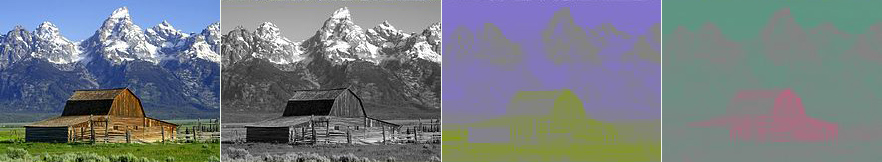
\includegraphics[width=0.9\textwidth]{./img/barn_rgb_ycc.jpg}
\captionof{figure}{Left RGB image, right the luminance and the 2 chrominance 
channels\cite{YCCWiki}}

\end{figure}

It is done using the transformation in \eqref{eq:ycc} and since our implementation was very inefficent, we used it as a preprocessing step rather than an online transformation. 
Unfortunately, the results were discouraging, the performance improved only slightly (below 1\%), which is below the fluctuations (due to random initalization and early stopping) we observed in various runs of identical models during the last assignment. Our explanation is that this is just a rather simple linear transformation of the input values, the network may already have done something similar on the first level. 




\section{Training the model}
After increasing the number of convolutional filters from the previous exercise we quickly had an improvement by $\approx 10\%$ in our validation accuracy. We employed different techniques to improve the validation accuracy from there but all efforts fell flat. 

\subsection{Dropout}
Dropout is a technique that counteracts overfitting in a model. It sets values of random neurons in the affected layer to zero with the specified probability. This forces the model to consider different features in the input to assign a certain class to the output (e.g. if the ``fur'' feature is dropped the model could predict that a cat is not a human based on features like ``has four legs'' combined with ``has a tail''). 


We first tried the same neural net architecture as in the previous assignment and quickly got a validation accuracy of approximately $80\%$ with a training accuracy of $>90\%$ -- we thought that applying measures to coutneract overfitting should increase the validation accuracy so we added dropout to the convolutional layers with varying probabilities (between $10\%$ and $30\%$) though this did not improve results.
though further modifications resulted in worse ($75\% - 80\%$) or even horrible results (all samples classified as the same class). 

We also tried applying dropout to the input layer, as this was recommended in the keras documentation. This will remove some of the input neurons. In our case, it did worsen the results and that seems plausible, since the input neurons are highly correlated and this is the same as adding random noise to the image, which of course will weaken the classification task. A better approach would be darkening whole parts of the image to simulate occlusion.

\section{Testing the model}
For the testing script, we applied a variant of the oversampling method described in the lecture. We test different versions of the image (flipped, cropped, rotated) against our model an added up the probabilities. For that we used the same transformation we already applied in the data augmentation part. To get the final class, we chose the one with the highest combined probability. We could not assess the quality improvements of this method, because by the time we implemented that the long queues on the server permitted experiments. But it is safe to say, that it wont worsen the results, so it is part of our testing method. We would also have liked to choose only those top results, that differ the most from each other, but again, without experimenting, this part was scraped.


